\documentclass{article}

\usepackage{tcolorbox}
\usepackage{ulem} %math
\usepackage{amsmath}
\usepackage{amsfonts}
\usepackage{amssymb}
\usepackage{graphicx}
\usepackage{enumerate}


%Create a box for theorems
%\begin{theo}[titel] %optional
%tekst
%\end{theo}
\newenvironment{theo}[1][Vigtigt]{%
\begin{tcolorbox}[colback=green!5,colframe=green!40!black,title=\textbf{#1}]
}{%
\end{tcolorbox}
}




%Create a square matrix
%\begin{ArgMat}{2}
%21 & 22 & 23 \\  
%a & b & c
%\end{ArgMat}
%
% Info: http://tex.stackexchange.com/questions/2233/whats-the-best-way-make-an-augmented-coefficient-matrix
%
\newenvironment{ArgMat}{%
$
  \left[\begin{array}{@{}*{100}{r}r@{}}
}{%
  \end{array}\right]
  $
}

\newenvironment{deter}{%
$
  \left|\begin{array}{@{}*{100}{r}r@{}}
}{%
  \end{array}\right|
  $
}


%Create multiple lines with holes
%\begin{SysEqu}
%x_1 && &- &5x_3 &+ &2x_4=& 1 \\
%x_1 &+ &x_2 &+ &x_3 && =& 4 \\
%&&&&&&0 =& 0
%\end{SysEqu}
\newenvironment{SysEqu}{%
$  \setlength\arraycolsep{0.1em}
  \begin{array}{@{}*{100}{r}r@{}}
}{%
  \end{array}$
}

%Create solution for x_1, x_n...
%\begin{solu}
%x_1 &= d \\
%x_2 &= e \\
%x_3 &= s
%\end{solu}
\newenvironment{solu}{%
$
  \setlength\arraycolsep{0.1em}
  \left\{\begin{array}{@{}*{100}{r}r@{}}
}{%
  \end{array}\right.
$
}

\usepackage{lastpage}


\newcommand{\HRule}{\rule{\linewidth}{0.8mm}}

%Tekst i fotter
\newcommand{\footerText}{\thepage\xspace /\pageref{LastPage}}
\newcommand{\ProjectName}{433 MHz styring af AeroQuad}


\chapterstyle{hangnum}




\nouppercaseheads
\makepagestyle{mystyle} 

\makeevenhead{mystyle}{}{\\ \leftmark}{} 
\makeoddhead{mystyle}{}{\\ \leftmark}{} 
\makeevenfoot{mystyle}{}{\footerText}{} 
\makeoddfoot{mystyle}{}{\footerText}{} 
\makeatletter
\makepsmarks{mystyle}{% Overskriften på sidehovedet
  \createmark{chapter}{left}{shownumber}{\@chapapp\ }{.\ }} 
\makeatother
\makefootrule{mystyle}{\textwidth}{\normalrulethickness}{0.4pt}
\makeheadrule{mystyle}{\textwidth}{\normalrulethickness}

\makepagestyle{plain}
\makeevenhead{plain}{}{}{}
\makeoddhead{plain}{}{}{}
\makeevenfoot{plain}{}{\footerText}{}
\makeoddfoot{plain}{}{\footerText}{}
\makefootrule{plain}{\textwidth}{\normalrulethickness}{0.4pt}

\pagestyle{mystyle}

%%----------------------------------------------------------------------
%
%%Redefining chapter style
%%\renewcommand\chapterheadstart{\vspace*{\beforechapskip}}
%\renewcommand\chapterheadstart{\vspace*{10pt}}
%\renewcommand\printchaptername{\chapnamefont }%\@chapapp}
%\renewcommand\chapternamenum{\space}
%\renewcommand\printchapternum{\chapnumfont \thechapter}
%\renewcommand\afterchapternum{\space: }%\par\nobreak\vskip \midchapskip}
%\renewcommand\printchapternonum{}
%\renewcommand\printchaptertitle[1]{\chaptitlefont #1}
\setlength{\beforechapskip}{0pt} 
\setlength{\afterchapskip}{0pt} 
%\setlength{\voffset}{0pt} 
\setlength{\headsep}{25pt}
%\setlength{\topmargin}{35pt}
%%\setlength{\headheight}{102pt}
%\setlength{\textheight}{302pt}
\renewcommand\afterchaptertitle{\par\nobreak\vskip \afterchapskip}
%%----------------------------------------------------------------------




%Sidehoved og -fod pakke
%Margin
\usepackage[left=2cm,right=2cm,top=2.5cm,bottom=2cm]{geometry}
\usepackage{lastpage}



%%URL kommandoer og sidetal farve
%%Kaldes med \url{www...}
%\usepackage{color} %Skal også bruges
\usepackage{hyperref}
\hypersetup{ 
	colorlinks	= true, 	% false: boxed links; true: colored links
    urlcolor	= blue,		% color of external links
    linkcolor	= black, 	% color of page numbers
    citecolor	= blue,
}



%Mellemrum mellem linjerne    
\linespread{1.5}


%Seperated files
%--------------------------------------------------
%Opret filer således:
%\documentclass[Navn-på-hovedfil]{subfiles}
%\begin{document}
% Indmad
%\end{document}
%
% I hovedfil inkluderes således:
% \subfile{navn-på-subfil}
%--------------------------------------------------
\usepackage{subfiles}

%Prevent wierd placement of figures
%\usepackage[section]{placeins}

%Standard sti at søge efter billeder
%--------------------------------------------------
%\begin{figure}[hbtp]
%\centering
%\includegraphics[scale=1]{filnavn-for-png}
%\caption{Titel}
%\label{fig:referenceNavn}
%\end{figure}
%--------------------------------------------------
\usepackage{graphicx}
\usepackage{subcaption}
\usepackage{float}
\graphicspath{{../Figures/}}

%Speciel skrift for enkelt linje kode
%--------------------------------------------------
%Udskriver med fonten 'Courier'
%Mere info her: http://tex.stackexchange.com/questions/25249/how-do-i-use-a-particular-font-for-a-small-section-of-text-in-my-document
%Eksempel: Funktionen \code{void Hello()} giver et output
%--------------------------------------------------
\newcommand{\code}[1]{{\fontfamily{pcr}\selectfont #1}}


% Følgende er til koder.
%----------------------------------------------------------
%\begin{lstlisting}[caption=Overskrift på boks, style=Code-C++, label=lst:referenceLabel]
%public void hello(){}
%\end{lstlisting}
%----------------------------------------------------------

%Exstra space
\usepackage{xspace}
%Navn på bokse efterfulgt af \xspace (hvis det skal være mellemrum
%gives det med denne udvidelse. Ellers ingen mellemrum.
\newcommand{\codeTitle}{Kodeudsnit\xspace}

%Pakker der skal bruges til lstlisting
\usepackage{listings}
\usepackage{color}
\usepackage{textcomp}
\definecolor{listinggray}{gray}{0.9}
\definecolor{lbcolor}{rgb}{0.9,0.9,0.9}
\renewcommand{\lstlistingname}{\codeTitle}
\lstdefinestyle{Code}
{
	keywordstyle	= \bfseries\ttfamily\color[rgb]{0,0,1},
	identifierstyle	= \ttfamily,
	commentstyle	= \color[rgb]{0.133,0.545,0.133},
	stringstyle		= \ttfamily\color[rgb]{0.627,0.126,0.941},
	showstringspaces= false,
	basicstyle		= \small,
	numberstyle		= \footnotesize,
%	numbers			= left, % Tal? Udkommenter hvis ikke
	stepnumber		= 2,
	numbersep		= 6pt,
	tabsize			= 2,
	breaklines		= true,
	prebreak 		= \raisebox{0ex}[0ex][0ex]{\ensuremath{\hookleftarrow}},
	breakatwhitespace= false,
%	aboveskip		= {1.5\baselineskip},
  	columns			= fixed,
  	upquote			= true,
  	extendedchars	= true,
 	backgroundcolor = \color{lbcolor},
	lineskip		= 1pt,
%	xleftmargin		= 17pt,
%	framexleftmargin= 17pt,
	framexrightmargin	= 0pt, %6pt
%	framexbottommargin	= 4pt,
}

%Bredde der bruges til indryk
%Den skal være 6 pt mindre
\usepackage{calc}
\newlength{\mywidth}
\setlength{\mywidth}{\textwidth-6pt}


% Forskellige styles for forskellige kodetyper
\usepackage{caption}
\DeclareCaptionFont{white}{\color{white}}
\DeclareCaptionFormat{listing}%
{\colorbox[cmyk]{0.43, 0.35, 0.35,0.35}{\parbox{\mywidth}{\hspace{5pt}#1#2#3}}}
\captionsetup[lstlisting]
{
	format			= listing,
	labelfont		= white,
	textfont		= white, 
	singlelinecheck	= false, 
	width			= \mywidth,
	margin			= 0pt, 
	font			= {bf,footnotesize}
}

\lstdefinestyle{Code-C} {language=C, style=Code}
\lstdefinestyle{Code-Java} {language=Java, style=Code}
\lstdefinestyle{Code-C++} {language=[Visual]C++, style=Code}
\lstdefinestyle{Code-VHDL} {language=VHDL, style=Code}
\lstdefinestyle{Code-Bash} {language=Bash, style=Code}

%Text typesetting
%--------------------------------------------------------
%\usepackage{baskervald}
\usepackage{lmodern}
\usepackage[T1]{fontenc}              
\usepackage[utf8]{inputenc}         
\usepackage[english]{babel}       

\setlength{\parindent}{0pt}
\nonzeroparskip

%\setaftersubsecskip{1sp}
%\setaftersubsubsecskip{1sp}
 


%Dybde på indholdsfortegnelse
%----------------------------------------------------------
%Chapter, section, subsection, subsubsection
%----------------------------------------------------------
\setcounter{secnumdepth}{3}
\setcounter{tocdepth}{3}


%Tables
%----------------------------------------------------------
\usepackage{tabularx}
\usepackage{array}
\usepackage{multirow} 
\usepackage{multicol} 
\usepackage{booktabs}
\usepackage{wrapfig}
\renewcommand{\arraystretch}{1.5}



%Misc
%----------------------------------------------------------
\usepackage{cite}
\usepackage{appendix}
\usepackage{amssymb}
\usepackage{url,ragged2e}
\usepackage{enumerate}
\usepackage{amsmath} %Math bibliotek


\usepackage{longtable}


\begin{document}
\section{Reactor Pattern}

The Reactor architectural pattern allows event-driven applications to demultiplex \& dispatch service requests that are delivered to an application from one or more clients.

Generelt:
\begin{itemize}
	\item Bruges primært til servere, der \textit{venter} på events.
	Den checker dog hele tiden på, om der er kommet noget nyt.
	\item \code{Reactor} håndtere events til forskellige processer
	\item Modtages synkront og serielt
	\item Hvert event sorteres af en \code{Multiplex}er (baseret på indhold) og uddeles af en \code{Dispatcher} til en process. 
	Alle applikationsspecifike funtioner udføres af specifikke \code{EventHandler}s.
	\item Inversion of Control bruges (dependency (interface) injection) og gøre koden generisk. Se \codeTitle \ref{lst:DI}.
\end{itemize}

Implementering:
\begin{itemize}
	\item Klassen \code{Reactor} bruger GoF Bridge pattern (pointer til implementering -- også kaldet \emph{pimpl idiom}, da der kun er én implementering). 
	\item Klassen \code{Reactor} bruges som en Singleton.
	\item Klassen \code{Demultiplexter}'s \code{select()} har "file descripter set"    parametre. 
	Disse checkes for \code{READ}, \code{WRITE}, exceptions og time outs.
\end{itemize}

Fordele:
\begin{itemize}
	\item Separation of concerns
	\item[] Afkobler \code{Demux} og \code{Dispatcher} fra applikationsspecifik kode
	
	\item Modularity and reuseability
	\item[] Hvert event er sit eget komponent.

	\item Portability
	\item[] \code{Reactor} er frakoblet low-level kode og kan bruges af højre levels.

	\item Har et super godt samspil med \code{Wrapper Facade} pattern til low-level.
\end{itemize}

Ulemper:
\begin{itemize}
	\item Semi-svær at debugge.
	\item Single-threaded applikationer standser \code{Reactor} til de er færdige.
\end{itemize}

Andet:
\begin{itemize}
	\item \code{Reactor} kan bruges på clienten, hvis denne har nogle faste mønstre der kan sendes og modtages data i.
	I modsætning til serveren vil den kun kalde \code{HandleEvent()} én gang og exite.
	\item Sammensæt med Acceptor pattern, således serveren kalder accepter, og den registrere et gyldigt event.
	\item \code{Proactor}\fxnote{Skriv om dette}
\end{itemize}

\begin{lstlisting}[caption=Bridge / interface injection, style=Code-C++, label=lst:DI]
Reactor(IClass *impl)
{ impl->getData(); }
\end{lstlisting}

\begin{figure}[hbtp]
\centering
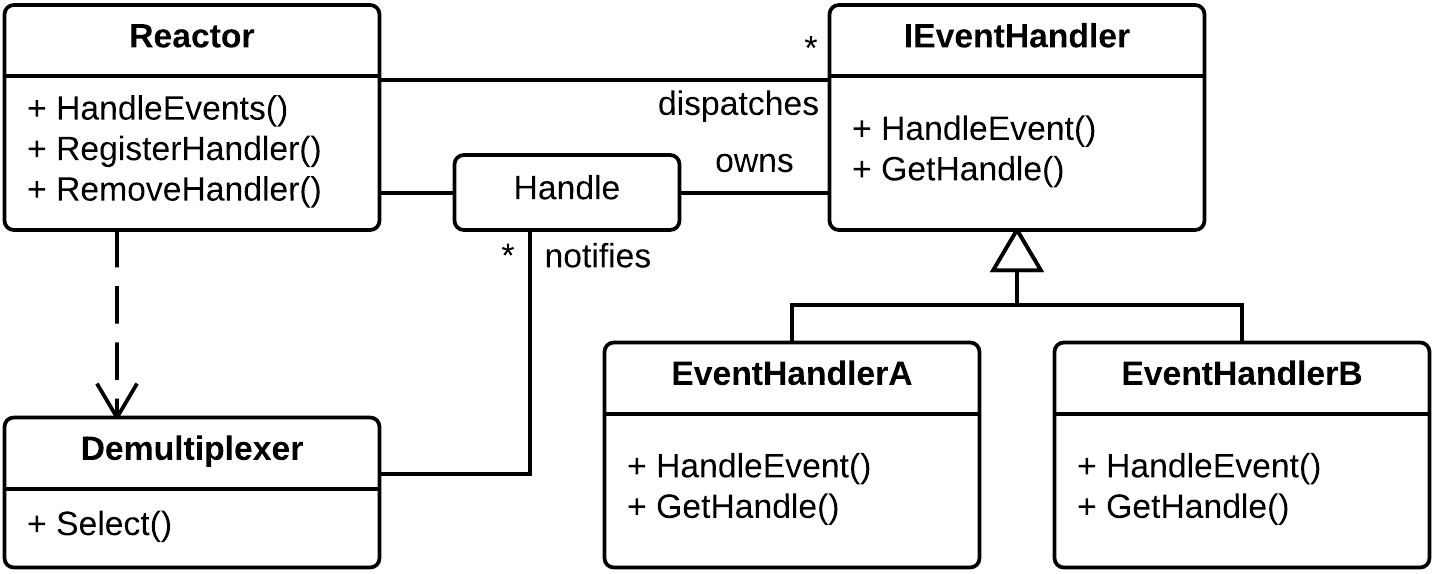
\includegraphics[width=0.9 \textwidth]{Reactor}
\end{figure}





\newpage
\section{Paradigms for Distributed Communication}

Space, time and flow:
\begin{itemize}
	\item Space decoupling betyder, at en publisher ikke kender til sine subscribers.
	Der er en service der klarer dette for den.

	\item Time decoupling betyder, at beskeder fra en publisher ikke skal komme per omgående til subscriber.
	Når først pubslisher udgiver, kan der gå tid til subscriber modtager.

	\item Flow decoupling betyder, at den forstyrrer når den vil?\fxnote{Check om dette er rigtigt}
\end{itemize}


RMI og publish/subscriber:
\begin{itemize}
	\item RMI -- Remote Method Invocation betyder, at du over et netværk kan aktivere en kommando, der bliver eksikveret (og muligvis sendt tilbage).

	\begin{itemize}
	 	\item Understøttes af Java, CORBA og Mircrosoft's DCOM
	 	\item Dur kun mellem 2 maskiner.
		\item Time og space er coupled :(
		\item Flow couple er meget stærk på consumer siden.
		\begin{itemize}
		 	\item Er ikke stærkt, hvis producer ikke forventer et svar
		 	\item Altså asynk
		 \end{itemize} 
	\end{itemize} 

	\item Publisher/Subscriber
	\begin{itemize}
		\item Decoupler space, time og flow ved at lade alt køre i en kanal (Socket/kø)
		\item The channel decouples
	\end{itemize}
\end{itemize}

\begin{figure}[ht]
\begin{minipage}[b]{0.45\linewidth}
\centering
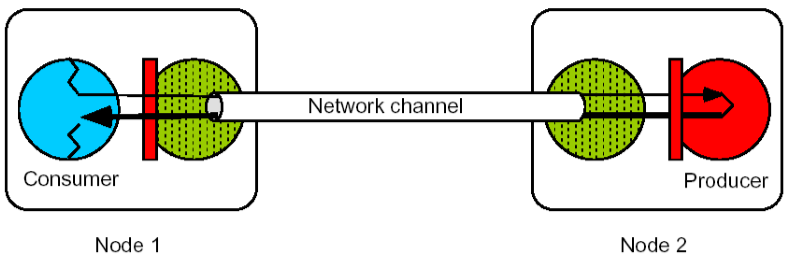
\includegraphics[width=\textwidth]{RMI}
\caption{RMI}
\label{fig:figure1}
\end{minipage} 						% No linebreak from here
\hspace{0.5cm}						% ...
\begin{minipage}[b]{0.45\linewidth}	% to here. They will over-under with linebreak
\centering
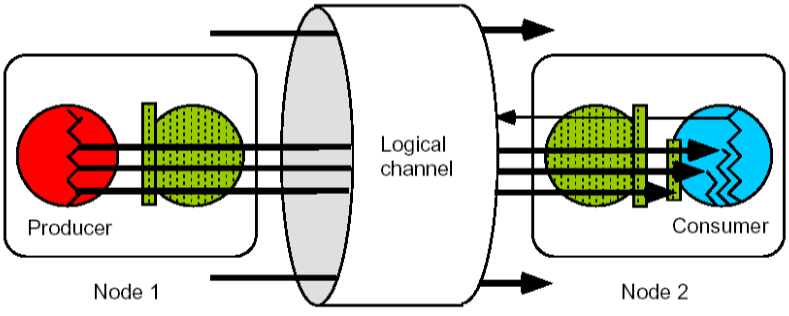
\includegraphics[width=\textwidth]{PS}
\caption{Publish/Subscribe}
\label{fig:figure2}
\end{minipage}
\end{figure}


Skal vi fortælle om de 3 versioner af p/s eller de andre, ringe løsninger?









\newpage
\section{Acceptor/Connector Pattern}


\subsection{Explain the "Acceptor/connector" pattern mechanism}
Acceptor-connector decoupler forbindelsen og services-laget.
Når først en forbindelse er accepteret, oprettes en seperat stream mellem de to.
Herefter vil \code{Reactor}'en (i et \code{while(1)}) bede \code{ServiceHandler}'en udføre sine opgaver.

Acceptor:
\vspace{-10pt}
\begin{itemize}
	\item Ligger på serveren.
	\item Modtager kun eventet \code{Accept()}  ment til den aktuelle \code{Acceptor}.
	\item Opretter konkrete \code{ServiceHandler}'re for events med \code{template}s  -- disse indeholder IP og port.
	\item Alle andre beskeder sendes direkte til \code{ServiceHandler} fra peer og aktiveres af \code{Dispatcher}'ens \code{HandleEvent()}.
\end{itemize}

Connector:
\vspace{-10pt}
\begin{itemize}
	\item Connector ligger på clienterne.
	\item Connectoren opretter en \code{ServiceHandler}, der snakker med Acceptorens \code{ServiceHandler}.
	\item Sender predefinere beskeder i form af \code{READ}, \code{WRITE} og \code{CONNECT} til serveren, hvor \code{CONNECT} binder \code{ServiceHandler}ne sammen.
	\item Beskederne sendes igennem en \code{ServiceHandler}en.
\end{itemize}



\subsection{Describe when to use an acceptor, a connector or both patterns in a node}
\begin{itemize}
	\item Acceptor bruges i alle servere, der har forskellige opgaver.
	Det vil forsimple besked-tilgangen og der kan oprettes seperate \code{ServiceHandler}e til forskellige connections.
	\item Connector bruges, hvis man har de tilsvarende beskeder til Acceptoren. 
	Dette vil sikre, at der ikke sendes beskeder der ikke må sendes?

	\item Brug begge i én node, når du ønsker p2p forbindelse i form af torrents and the likes.
\end{itemize}



\subsection{Describe the difference between a synchronous and an asynchronous connector}
Synkron:
\vspace{-10pt}
\begin{itemize}
	\item 
\end{itemize}

Asynkron:
\vspace{-10pt}
\begin{itemize}
	\item Clienter der har langsom forbindelse får ikke serveren til at vente.
	\item Clienter der er single-threaded kigger blot i en kø 
	\item Hvis (p2p) clienten har mange peers, som kobler til i tilfældig orden.
	\item Bruges sammen med en Proactor
	\item Generelt mange forbindelser vil 
\end{itemize}







\newpage
\section{Proactor and ACT Patterns}

\subsection{Explain the "Proactor" pattern mechanism and its interaction with the  
Asynchronous Completion Token (ACT) pattern}

Asynchronous Completion Token (ACT):
\vspace{-10pt}
\begin{itemize}
	\item Design pattern.
	\item Tillader effiktiv demultiplx og processering ved asynkrone operationer.
	\item Vil ved færdiggørelse returnere ACT (og resultat).
\end{itemize}

Proaktor:
\vspace{-10pt}
\begin{itemize}
	\item Erstatter \code{Reactor} som dispatcher.
	\item Sætter asynk-tråde til at udfører store opgaver og fortsætter med mindre i mellemtiden.
	\item Når en asynk bliver færdig, skubbes denne ind i en event-kø. 
	\item Denne gør Proactoren opmærksom på, at det er færdig og skubbes frem i køen af \code{HandleEvent()}.
	\item Herefter sendes dette videre til en \code{CompletionHandler} (det samme som ServiceHandler).
\end{itemize}


\subsection{Describe for what and when these pattern are used}

Proactor:
\vspace{-10pt}
\begin{itemize}
	\item Ved long-duration oprerationer, der eksikveres asynk.
	\item Hvis man derimod lader en asynk tråd håndtere lange kald, kan små kald passere imens. (forstil dig noget MatLab kode skal køre).
\end{itemize}


\subsection{Describe the benefits in comparison with the use of a Reactor pattern in combination with a concurrency pattern}


\begin{itemize}
	\item I reaktor pattern skal alt håndteres på lige fod. Det skal proactor ikke.
	\item Der er bedre OS portablility.
	\item Der laves færre tråde, da nogle \code{CompletionHandler}s ikke behøver tråde (alle concurrency vil).
	\item Dette undlader context switching.
\end{itemize}






\newpage
\section{Architecture Trade Off Method (ATAM) and Architecture Documentation}

\subsection{Describe for what and when the ATAM method is used}
\begin{itemize}
	\item ATAM (Architecture Trade off Analysis Method) er en metode til at checke, om systemet opfylder requirements.
	\begin{itemize}
		\item Funktionelle (main input til domain modellen)
		\item Ikke-funktionelle 
		\begin{itemize}
			\item Distribueret.
			\item Portabel.
			\item Oppe så mange \% af tiden.
			\item Sikker mod hackere.
			\item Minimum så hurtig.
		\end{itemize}
	\end{itemize}
	\item Skal overvejes, når man laver system architecturen.
\end{itemize}


\subsection{Explain the ATAM method steps}

Elicitation:
\vspace{-10pt}
\begin{enumerate}
	\item Saml scenarier for system brug fra repræsentative stakeholders.
	\item Saml krav, begrænsninger og omgivelser.
	\item Beskriv Architectural Views (flere -- der skal kunne opfylde de vigtige kvalitets krav).
	\item Lav Attribute-specific analysis.
	\item Find sensitive punkter.
	\item Find trade offs.
\end{enumerate}

Evaluering:
\vspace{-10pt}
\begin{enumerate}
	\item Presenter ATAM.
	\item Presenter business driver (forretningsmodel?).
	\item Presenter architecture.
	\item Find og prioriter ikke-funktionelle krav.
	\item Alternativer:
	\begin{itemize}
	 	\item Find alternative arkitekturtilgange.	
	 	\item Analyser det
		\item Præsenter resultat.
		\item Lav risk-analyse.
	 \end{itemize} 

	\item Lav rationelle valg (dokumenteret).
\end{enumerate}

\subsection{Describe the purpose of Architecture View Models and the relation to ATAM}

\begin{itemize}
	\item Architecture View Models har samme formål.
	\item AVM er lavet i flere omgange med $N+1$.
	\item $+1$ er scenarie/UC view.
	\item Alle indholder noget der viser komponentsammensætningen i lag, hvilke tasts der skal køre og hvordan hardwaren skal være.
	\item Nogle viser sikkerhed, nogle distribuere modeller, nogle de enkelte klasser.
\end{itemize}











\newpage
\section{Leader/Followers Pattern and Half sync/half async Pattern}

\subsection{Explain the "Leader/followers" pattern mechanism}
Metafor:
\vspace{-10pt}
\begin{itemize}
	\item Du vil med en taxa og skal tage den første.
	\item Denne taxa udfører en opgave.
	\item Den næste taxa er nu først.
	\item Når den førstenævnte taxa er færdig, stiller den sig bag i køren af taxa'er.
\end{itemize}

Mekanismen:
\vspace{-10pt}
\begin{itemize}
	\item Opret en pool af tråde, som alle kan gøre det samme.
	\item Vælg én som leader, giv denne den første opgave asynk og lad den næste blive promoveret.
	\item Når en tråd er færdig kalder den \code{Join()}\fxnote{Er det join()?} på \code{TreadPool} og sover til den bliver leader.
\end{itemize}


\subsection{Explain the main structure of the "half sync/half async" pattern the half sync/half async pattern}

\begin{itemize}
	\item Har synkrone og asynkrone tråde.
	\item Disse skal kunne snakke sammen.
	\item Imellem er en kø (singleton eller en kø pr service), som \code{read/write}- og \code{dequeue/enqueue}-operationer ligges i.
	\item Database kørsel i synkrone, separate tråde.
	\item Små, interrupt protokoller i asynkrone tråde.
	\item Vælg buffer strategi:
	\begin{itemize}
		\item FIFO
		\item Prioritet
		\item Notification 
	\end{itemize}
\end{itemize}


\subsection{Describe the advantages of the Leader/Followers pattern in comparison with the half sync/half async pattern}

Leader/Follow over half sync/async:
\vspace{-10pt}
\begin{itemize}
	\item LF har ikke brug for en buffer imellem sine tråde.
	\item Der er ikke et locking overhead mellem tråde.
	\item Simplere at implementere
\end{itemize}

Half sync/async over Leader/Follow:
\vspace{-10pt}
\begin{itemize}
	\item Kan nemmer implementere forskellige prioriteringsalgoritmer
	\item Kun én tråd kan demultiplex'e ad gangen.
\end{itemize}





\newpage
\section{Interceptor Pattern}

\subsection{Explain the "Interceptor" pattern mechanism}
\begin{itemize}
	\item Det kan tilføje services on-the-fly til et framework og aktiveres på et event.
	\item Disse kan tilgå frameworket, hvis de får tilsendt klassernes pointere.
\end{itemize}


\subsection{Describe how the interceptor can be used in developing a framework and the division of responsibilities between developers}


\subsection{Describe benefits and liabilities}




\newpage
\section{JAWS Framework}

\subsection{Explain the overall architecture of the JAWS-frameworket and how it is designed based on POSA2, POSA1 and GoF patterns}


\subsection{Describe the reconfiguration possibilities in JAWS}


\subsection{Describe the purpose of the used POSA2 design patterns}




\newpage
\section{Component Configurator Pattern}

\subsection{Explain the "Component Configurator" pattern mechanism}


\subsection{Describe how it can support dynamic reconfiguration at run-time}


\subsection{Describe benefits and liabilities}


































\end{document}